
\section{Introduction}
\begin{frame}
  \begin{center}
    Part I - Introduction
  \end{center}
\end{frame}

\begin{frame}{Lecture Outline}
  In the last lecture, we talked about how experiments are important for the scientific endeavor. In this lecture, we will focus on basic concepts and techniques for representing experimental data.\bigskip

  \begin{itemize}
    \item The importance of characterizing your data;
    \item Statistical Concepts: Population and Sample;
    \item Characterizing a Population: Point Estimators and Interval Estimators;
    \item Visualizing Estimators;
  \end{itemize}
\end{frame}

\subsection{Charles Darwin}
% To illustrate the importance of how to present your
% Research results, let's talk about one researcher
% whose research was all about collecting and displaying data,
% Charles Darwin

\begin{frame}{Charles Darwin}{1809--1882 British Naturalist, Geologist, Biologist}
  To open our discussion about data, let's talk about a scientist whose work was all about collecting and understanding lots of data.
  \bigskip

  \begin{columns}
    \column{.2\textwidth}
    \includegraphics[width=1\textwidth]{../img/irasutoya_darwin}
    \ppagenote{Charles Darwin sketch from \url{https://www.irasutoya.com}}
    \column{.8\textwidth}
    \begin{itemize}
      \item Well known for his theory on \structure{the origin of species}
      \item His theory correctly predicted the hereditary nature of evolution, even before genes were known.
      \item Actually, in his period, many people were interested in understanding the origin of the species;
    \end{itemize}
  \end{columns}
\end{frame}

\begin{frame}{Charlis Darwin}{Early Life}
  % Image: Child Darwin, wikipedia
  \hfill\includegraphics[width=.2\textwidth]{../img/wikipedia_darwinchild}
  \ppagenote{Charles Darwing Portrait from wikipedia (Public Domain)}
  \bigskip

  \begin{itemize}
    \item Son of a wealthy doctor in a large family;
    \item Apprenticed as a doctor, but found the classes dull.
    \item Prefered to learn \structure{taxidermy}, and catalog animals;
  \end{itemize}
\end{frame}

\begin{frame}{Charles Darwin}{Observing the World}
  % Image - HMS Beagle trip, wikipedia
  \begin{itemize}
    \item 1831: After graduation, went on a 5 year sea voyage to catalog geological and animal samples in South America and Asia;\medskip

    \item During the trip, he kept extensive notes of his observations and theories;\medskip

    \item His observations about the diversity of mockingbirds, tortoises, and foxes gave him new insights about the origin of the species;
  \end{itemize}\bigskip

  \begin{center}
    \includegraphics[width=.6\textwidth]{../img/wikipedia_darwin_beagle}
  \end{center}
\end{frame}

\begin{frame}{Charles Darwin}{On the Origin of the Species}
  % Image: The origin of the species
  \begin{columns}
    \column{0.2\textwidth}
    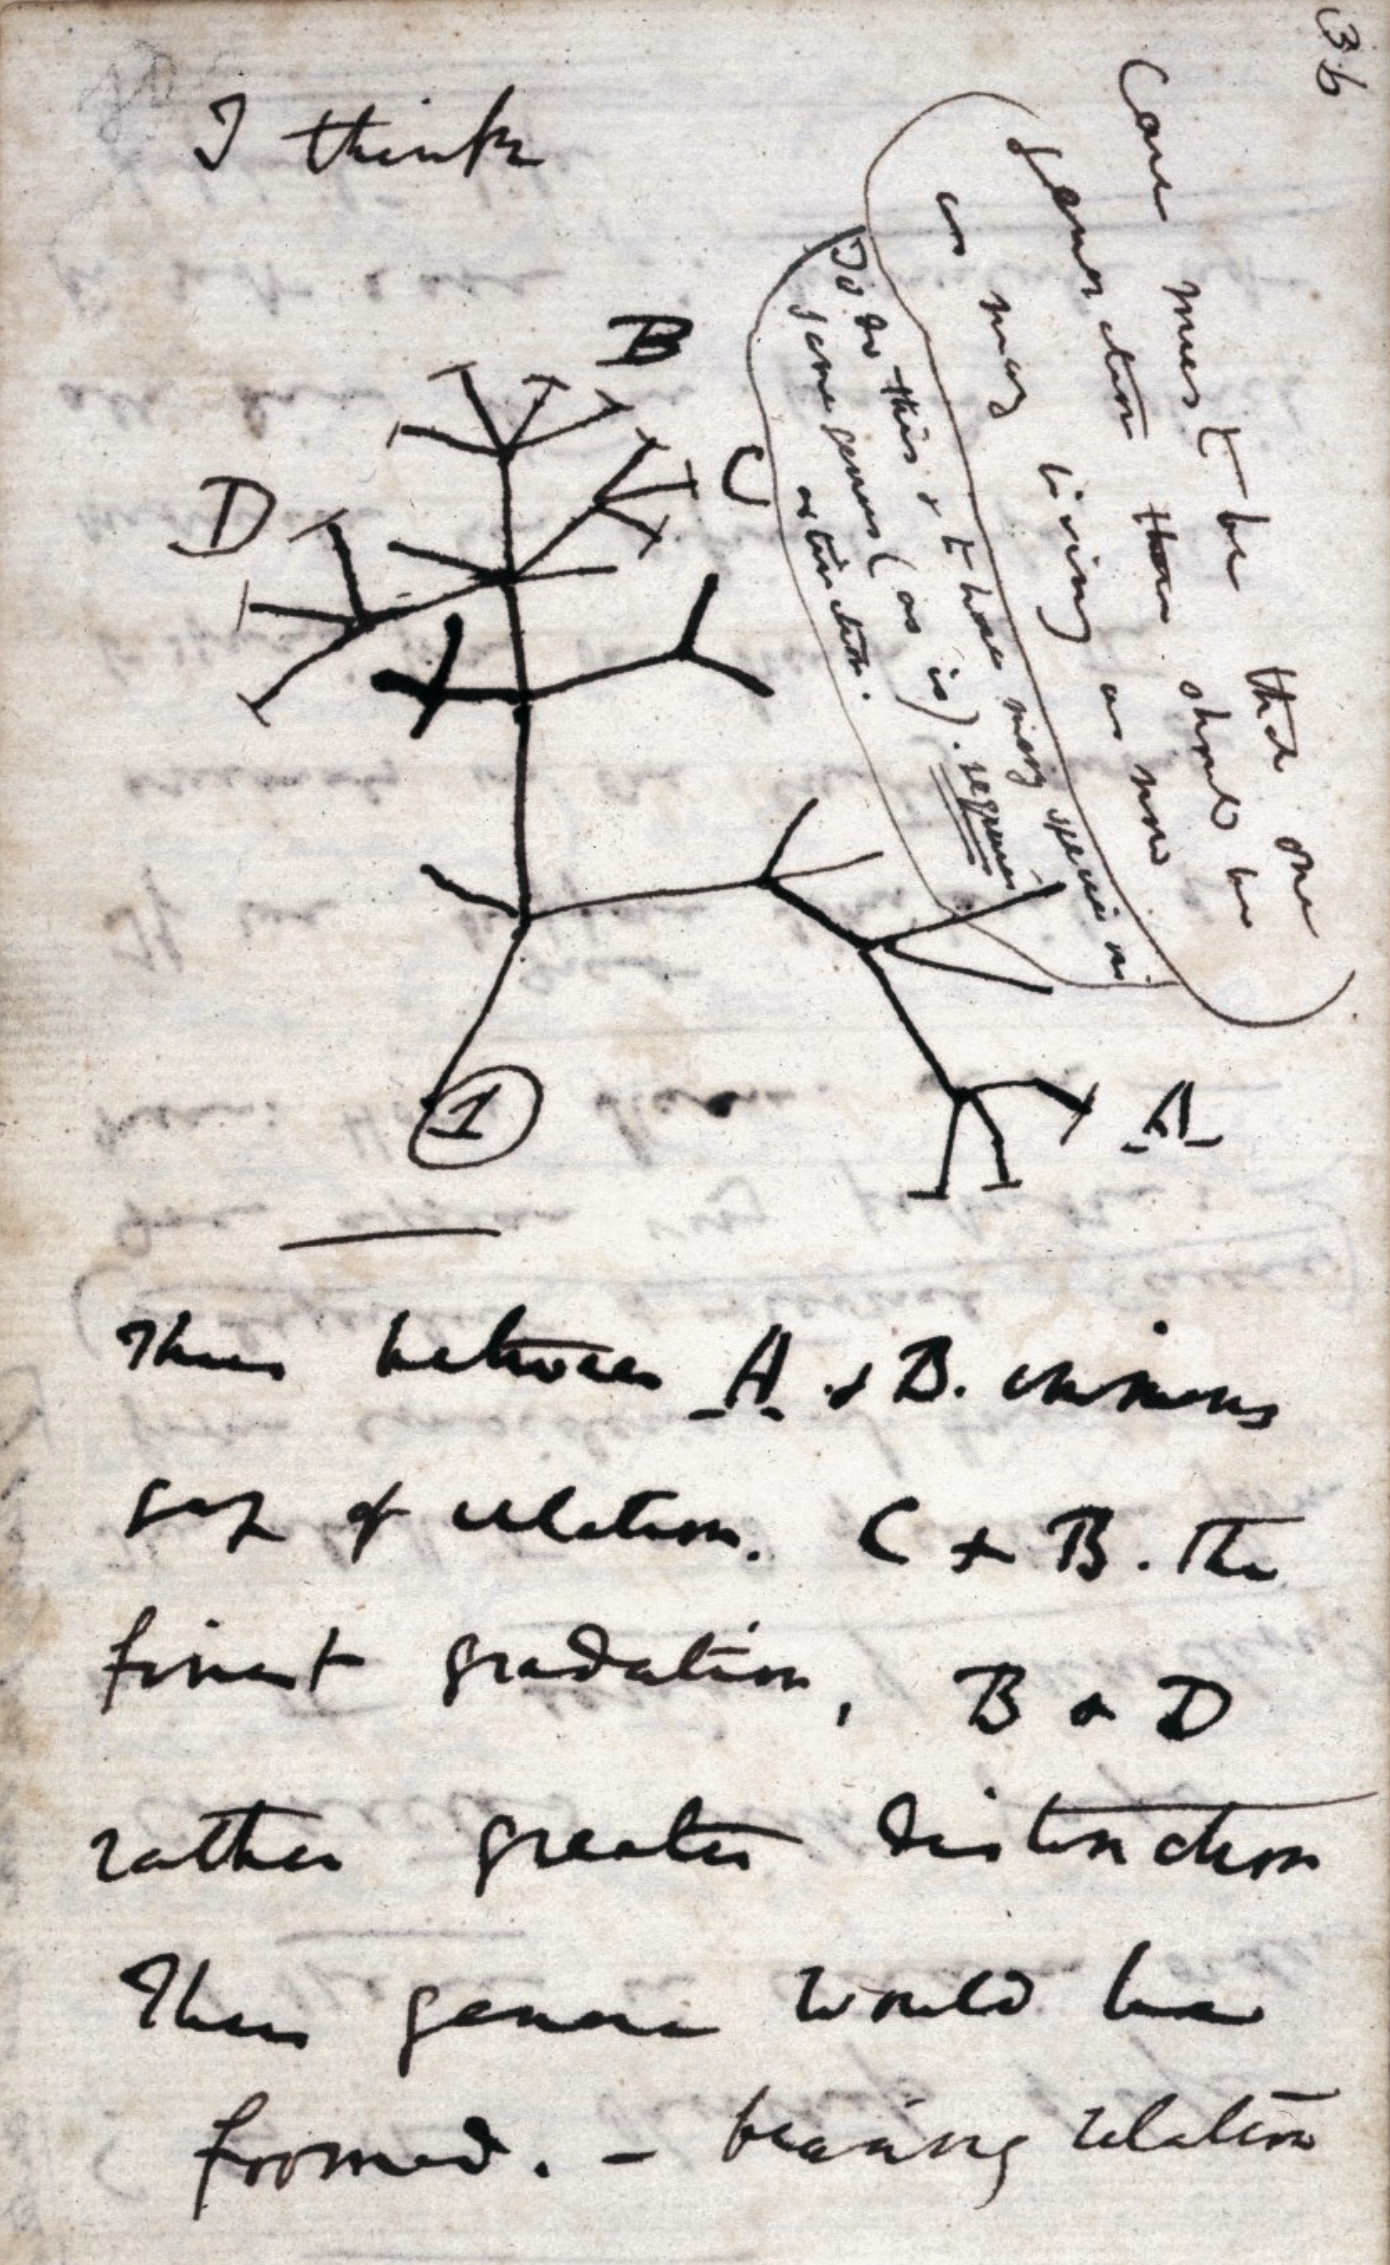
\includegraphics[width=1\textwidth]{../img/wikipedia_darwin_manuscript}
    \column{0.8\textwidth}
  \begin{itemize}
    \item In 1837, his notes from the Beagle's trip gave him his first insights about how "one species transforms into another"
    \item He gathered more and more data to confirm his theory, from marine biologists, farmers and breeders, plants, etc.
    \item This task of cataloguing and experimenting took over 15 years;
    \item Eventually published "On The Origin of the Species" in 1859, by encouragement from his friend scientists;
  \end{itemize}
  \end{columns}
\end{frame}

\begin{frame}{A note about programming language}
  Starting from this lecture, I will show some coding examples using the \structure{R programming language}. I highly recommend students in this course to get used to R. Read the following link if for one nice tutorial:\bigskip

  R for Beginners: \url{https://cran.r-project.org/doc/contrib/Paradis-rdebuts_en.pdf}\bigskip

  I also recommend the use of \structure{R Studio} for working with R, instead of working directly in the command prompt. \url{https://rstudio.com}
  \vfill

  \hfill\includegraphics[width=.2\textwidth]{../img/Rlogo}
\end{frame}


\section{Indicators}
\begin{frame}
  \begin{center}
    Part II - Indicators
  \end{center}
\end{frame}

\begin{frame}{Using data to characterize a system}
  In the last lecture, we talked about using experiments to obtain data.
  How can we use the data to gain \structure{knowledge} about a system?
  \bigskip


  \begin{columns}
    \column{0.8\textwidth}
    For example, let's say that we measure the \structure{height of one student}. Can I use this information to say something about the
    \structure{height of all students} in the university?
    \column{.2\textwidth}
    \includegraphics[width=\textwidth]{../img/irasutoya_height}
    \ppagenote{Height image from \url{https://www.irasutoya.com}}
  \end{columns}
\end{frame}

\begin{frame}{Using data to characterize a system}
  From a single student's height, it seems hard to learn anything about
  the height of the students of the university {\bf in general}.
  A better approach would be to take the height of several students.\bigskip

  \begin{center}
    \includegraphics[width=0.1\textwidth]{../img/irasutoya_height}
    \includegraphics[width=0.1\textwidth]{../img/irasutoya_height}
    \includegraphics[width=0.1\textwidth]{../img/irasutoya_height}
    \includegraphics[width=0.1\textwidth]{../img/irasutoya_height}
    \includegraphics[width=0.1\textwidth]{../img/irasutoya_height}
    \includegraphics[width=0.1\textwidth]{../img/irasutoya_height}
    \includegraphics[width=0.1\textwidth]{../img/irasutoya_height}
    \includegraphics[width=0.1\textwidth]{../img/irasutoya_height}
  \end{center}
  \bigskip

  If I calculate the \structure{average height} of several students, what is the relationship between this value and height of students in general?
\end{frame}

\subsection{Basic Concepts}
\begin{frame}{Population and Sample}
  This example introduces us to the concepts of statistical \structure{Population} and \structure{Sample}.\bigskip

  \begin{itemize}
    \item {\bf Population}: It is a large set of objects that are of interest as a whole. It can be a real set (all students in a university) or a theoretical set (all possible results of an experiment).\medskip

    \item {\bf Observation}: It is one element from the population. One student from the university, or one execution of an experiment.\medskip

    \item {\bf Sample}: It is a subset of the population. By examining the sample, we can \structure{make inferences} about the population as a whole.
  \end{itemize}
  \bigskip

  "Making inferences of the population from the sample". What does it mean?
\end{frame}

\begin{frame}{Population and Sample}{Making Inferences from the sample}
  \begin{block}{Population}
    \begin{columns}
      \column{.18\textwidth}
      \includegraphics[width=1\textwidth]{../img/ballpool}
      \column{.65\textwidth}
      A pool has many colorful balls. If you knew exactly how many, you could calculate the \structure{probability} of picking a ball of a certain color at random. {\bf But you don't know!}
    \end{columns}
  \end{block}
  \begin{block}{Sample}
    \begin{columns}
      \column{.14\textwidth}
      \includegraphics[width=1\textwidth]{../img/ballhand}
      \column{.65\textwidth}
      It is possible to {\bf estimate} the proportion of balls in the pool. To do that, we pick up a number of balls, and examine the \structure{proportion of the sample}.
    \end{columns}
  \end{block}

  \structure{CS Example:} Estimate total transfer time of
  a large file from the arrival time of a sample of packets.
  What could go wrong?
\end{frame}

\begin{frame}{Population and Parameters}
  \begin{columns}
    \column{0.5\textwidth}
      Our usual goal when obtaining and analysing experimental data is to estimate values for \structure{parameters} of the population.\bigskip

      A {\bf parameter} $\theta$ of the population is an unknown value of interest that characterizes some important aspect for our research.\bigskip

      Because we cannot observe the population directly, we have to estimate the parameter's true value from information gathered from the sample.
    \column{0.5\textwidth}
    \includegraphics[width=1\textwidth]{../img/wikipedia_triceratops}
    \ppagenote{Triceratops information table CC by Zachi Evenor and MathKnight}
  \end{columns}
\end{frame}



\begin{frame}{Samples and Statistics}
  By observing data obtained from a sample, we can {\bf characterize} (estimate) parameters from a population of interest. For example:\bigskip

  \begin{itemize}
    \item We calculate the average of the running time of multiple executions of a program, and estimate the mean running time;
    \item We ask the age of several students in a school, and estimate the maximum and minimum age of the students;
    \item We estimate the efficacy of a remedy by counting what percentage of patients get better after drinking it;
    \item We determine which of two neural networks is more precise by subtracting the test error of the two networks from each other;
  \end{itemize}\bigskip

  \begin{block}{Statistic}
    A statistic is a {\bf function} calculated from data obtained from a sample.
  \end{block}
\end{frame}

\begin{frame}{Errors and Biases}
  Note that we are being very careful to always use the word {\bf estimate} when we talk about statistics. Why is that?
  \bigskip

  In all the examples that we mentioned, if we are unlucky\footnote{or careless, or malicious}, we could obtain an estimate that is very different from the true value of the population:
  \begin{alertblock}{Bad statistics example}
    To estimate the height of the students of a school, we pick 10 students, and we measure the height of the youngest one.
  \end{alertblock}\medskip
  \begin{itemize}
    \item {\bf Error}: The difference between an estimate and the true value of a population's parameter;
    \item {\bf Bias}: The property of a statistic that systematically produces wrong estimates;
  \end{itemize}
\end{frame}

\begin{frame}{Point and Interval Indicators}
  The idea of estimating parameters of a population using information
  obtained from a sample is called {\bf statistical inference}.
  \bigskip

  In this lecture, we will focus on two central concepts of statistical inference: {\bf Point Estimators} and {\bf Interval Estimators}.\bigskip

  \begin{itemize}
    \item {\bf Point Estimators}: are statistics that estimate the value of a population parameter from information in a sample;

    \item {\bf Interval Estimators}: are statistics that estimate a \structure{range of values} of a population parameter from information in a sample;
  \end{itemize}
\end{frame}

\begin{frame}{Statistics and Sampling Distributions}
  Suppose that you want to obtain a point estimate for an arbitrary parameter of the population (e.g. mean size);\medskip

  Random samples of the population can be interpreted as a {\bf random variable}, and any function of these samples (any statistic) will
  be a random variable as well.\medskip

  \begin{columns}
    \column{.3\textwidth}
      \includegraphics[width=1\textwidth]{../img/sampling_distribution}
    \column{.7\textwidth}
      As a random variable, any statistic also has its own \structure{probability distribution}, called {\bf sampling distribution}.\bigskip

      Most statistical tests use properties of the sampling distributions (which are not the same as the true distribution of the population). We will talk more about those later.
  \end{columns}

\end{frame}

%% TODO: this part was taken directly from campelo's materials, Needs update.
\subsection{Point Indicators}
\begin{frame}{Definition of Point Indicator}
  A \emph{point estimator} is a statistic which provides the value of maximum plausibility for an (unknown) population parameter $\theta$.
  \bigskip

  Consider a random variable $X$ distributed according to a given $f(X|\theta)$.\bigskip

  Consider also a random sample from this variable: $x=\{x_1,x_2,\ldots,x_n\}$;\bigskip

  A given function $\hat{\Theta}=h\left(x\right)$ is called a \emph{point estimator} of the parameter $\theta$, and a value returned by this function for a given sample is referred to as a \emph{point estimate} $\hat{\theta}$ of the parameter.
\end{frame}

%% TODO: this part was taken directly from campelo's materials, Needs update.
\begin{frame}{Examples}
Point estimation problems arise frequently in all areas of science and engineering, whenever there is a need for estimating, e.g.,:\bigskip

\begin{itemize}
  \item a population  mean, $\mu$;
	\item a population variance, $\sigma^2$;
	\item a population proportion, $p$;
	\item the difference in the means of two populations, $\mu_1-\mu_2$;
	\item etc..
\end{itemize}\bigskip

In each case there are multiple ways of performing the estimation task, and the decision about which estimators to use is based on the mathematical properties of each statistic.
\end{frame}


%% TODO: this part was taken directly from campelo's materials, Needs update.
\begin{frame}{Unbiased estimators}
A good estimator should consistently generate estimates that lie close to the real value of the parameter $\theta$.\bigskip

A given estimator $\hat{\Theta}$ is said to be \textit{unbiased} for parameter $\theta$ if:\bigskip

\begin{equation*}
E\left[\hat{\Theta}\right] = \theta
\end{equation*}
\noindent or, equivalently:
\begin{equation*}
E\left[\hat{\Theta}\right] - \theta = 0
\end{equation*}\bigskip

The difference $E\left[\hat{\Theta}\right] - \theta$ is referred to as the \textit{bias} of a given estimator.
\end{frame}

%% TODO: this part was taken directly from campelo's materials, Needs update.
\begin{frame}{Unbiased estimators}
For example, the usual estimators for mean is an unbiased estimator;
\bigskip

Let $x_1,\ldots,x_n$ be a random sample from a given population $X$, characterized by its mean $\mu$ and variance $\sigma^2$. In this situation, it is possible to show that:
\bigskip

\begin{equation*}
E\left[\bar{x}\right] = E\left[\frac{1}{n}\sum\limits_{i=1}^{n}x_i\right] = \mu
\end{equation*}
\vfill

(Remember that the expected value of one observation is the mean value of the population)

\end{frame}

%% TODO: this part was taken directly from campelo's materials, Needs update.
\begin{frame}{Unbiased estimators}

Fora a population parameter $\theta$, it is usually possible to define more than one unbiased estimator. The variances of these estimators may, however, be different\bigskip

\begin{columns}[T]
    \column{0.5\textwidth}\vspace{-1.5em} \includegraphics[width=1\textwidth]{../img/unbiased_variance.png}
    \column{0.5\textwidth} In these cases, we usually want to obtain the unbiased estimator of minimal variance. This is generally called the \textit{minimal-variance unbiased estimator} (MVUE).
\end{columns}\bigskip

MVUE are generally chosen as estimators due to their ability of generating estimates $\hat{\theta}$ that are (relatively) close to the real value of $\theta$.
\ppagenote{Image: D.C.Montgomery,G.C. Runger, \textit{Applied Statistics and Probability for Engineers},Wiley 2003.}
\end{frame}


%% TODO: this part was taken directly from campelo's materials, Needs update.
\begin{frame}{Standard error of a point estimator}
Remember that because a point estimator is a random variable, it has an associated distribution and error. For example, the standard error of an estimator $\hat{\Theta}$ is
\begin{equation*}
\sigma_{\hat{\Theta}} = \sqrt{Var\left[\hat{\Theta}\right]}
\end{equation*}\bigskip

However, we can't know this directly. We can {\bf estimate} the standard error of the estimator from the data in the sample. In this case, we refer to it as the \textit{estimated standard error}, $\hat{\sigma}_{\hat{\Theta}}$ (the notations $s_{\hat{\Theta}}$ and $se(\hat{\Theta})$ are also common).

\hfill\includegraphics[width=.1\textwidth]{../img/yodawg}
\end{frame}

%% TODO: this part was taken directly from campelo's materials, Needs update.
\begin{frame}{Standard error of a point estimator}{Examples}
  Assuming a random variable $X$ from a gaussian distribution, and a sample error $s$, we can calculate the standard errors of several common point indicators\footnote{See Ahn and Fessler (2003), \textit{Standard Errors of Mean, Variance, and Standard Deviation Estimators}: \url{https://git.io/v5Z5v}}

\begin{equation*}
\hat{\sigma}_{\bar{X}} = \frac{s}{\sqrt{n}}
\end{equation*}

\begin{equation*}
\hat{\sigma}_{S^2} = s^2\sqrt{\frac{2}{n-1}}
\end{equation*}

\begin{equation*}
\hat{\sigma}_{S} = \frac{s}{\sqrt{2(n-1)}} + O\left(\frac{1}{n\sqrt{n}}\right)\approx \frac{s}{\sqrt{2(n-1)}}
\end{equation*}\bigskip
\end{frame}

\begin{frame}{Point Estimator Use Case}
  \includegraphics[width=.4\textwidth]{../img/pixabay_cable}
  \ppagenote{Coaxial cable image from \url{https://pixabay.com}}
  \bigskip

  Consider an operation to produce coaxial cables\footnote{Example inspired on \url{https://www.sas.com/resources/whitepaper/wp_4430.pdf}}. The mean resistance of the production is $50\Omega$, with a standard deviation of $2\Omega$ (Population mean, and population deviation).\bigskip

  Let's assume that the resistance value of the produced cables are distributed follow a normal distribution ($X\sim\mathcal{N}\left(\mu=50,\sigma^2=4\right)$)
\end{frame}

\begin{frame}{Point estimator use case}
  \begin{columns}
    \column{.35\textwidth}
    \includegraphics[width=1\textwidth]{../img/pixabay_cable}
    \column{.65\textwidth}
    Suppose that we take a random sample of $25$ cables is taken from
    this production process (an experiment, to measure if the process
    is correct, for example).
  \end{columns}
  \bigskip
The \structure{sample mean} of the the observations is:
\begin{equation*}
\bar{x} = \frac{1}{25}\sum\limits_{i=1}^{25}{x_i}
\end{equation*}

The \structure{sample mean} follows a normal distribution, with $E[\bar{x}] = \mu = 50\Omega$\footnote{since the sample mean is an unbiased estimator} and $\sigma_{\bar{x}} = \sqrt{\sigma^2/25} = 0.4\Omega$. The error depends on the sample size.
\end{frame}


\subsection{The Central Limit Theorem}

%% TODO: this part was taken directly from campelo's materials, Needs update.
\begin{frame}{The Central Limit Theorem}
In the previous example, the production operation followed a normal distribution. But even for a population with an arbitrary distribution, the sampling distribution of its mean tends to be approximately normal.
%(with $E[\bar{x}] = \mu $ and $s_{\bar{x}} = \sigma^2/n$).
\bigskip

More generally, let $x_1,\ldots,x_n$ be a sequence of \textbf{independent and identically distributed} (\textbf{iid}) random variables, with mean $\mu$ and finite variance $\sigma^2$. Then:
\begin{equation*}
z_n = \frac{\sum\limits_{i=1}^{n}{(x_i)} - n\mu}{\sqrt{n\sigma^2}} = \frac{\bar{x} - \mu}{\sqrt{\sigma^2/n}}
\end{equation*}

is distributed asymptotically as a standard Normal variable, that is, $z_n\sim\mathcal{N}(0,1)$.
\end{frame}

%% TODO: this part was taken directly from campelo's materials, Needs update.
\begin{frame}
{The Central Limit Theorem}
This result is known as the \textit{Central Limit Theorem}\footnote{For more details on the CLT, see \url{https://www.encyclopediaofmath.org/index.php/Central_limit_theorem}}, and is one of the most useful properties for statistical inference. The CLT allows the use of techniques based on the Normal distribution, even when the population under study is not normal.\bigskip

For ``well-behaved'' distributions (continuous, symmetrical, unimodal - the usual bell-shaped pdf we all know and love) even small sample sizes are commonly enough to justify invoking the CLT and using parametric techniques.\bigskip
\end{frame}

\begin{frame}
{Sampling Distributions}
{The Central Limit Theorem}
For an interactive demonstration of the CLT, download the files in {\small\url{https://git.io/vnPj8}} and run on RStudio.
\bigskip

{\centering\includegraphics[width=\textwidth]{../img/CLTdemo.png}}
\end{frame}

\subsection{Confidence Interval}
%% TODO: need to review the entire section

\begin{frame}{Statistical Intervals}
Statistical intervals are important in quantifying the uncertainty associated to a given estimate;
\bigskip

As an example, let's recap the coaxial cables example: \textit{a coaxial cable manufacturing operation produces cables with a target resistance of $50\Omega$ and a standard deviation of $2\Omega$. Assume that the resistance values can be well modeled by a normal distribution}.
\bigskip

Let us now suppose that a sample mean of $n=25$ observations of resistance  yields $\bar{x} = 48$. Given the sampling variability, it is very likely that this value is not exactly the true value of $\mu$, but we are so far unable quantify how much uncertainty there is in this estimate.
\end{frame}

%=====

\begin{frame}{Definition}
\textit{Statistical intervals} define regions that are likely to contain the true value of an estimated parameter.
\bigskip

More formally, it is generally possible to quantify the level of uncertainty associated with the estimation, thereby allowing the derivation of sound conclusions at predefined levels of certainty.
\bigskip

Three of the most common types of interval are:

\begin{itemize}
  \item Confidence Intervals;
  \item Tolerance Intervals;
  \item Prediction Intervals;
\end{itemize}
\end{frame}


%=====

\begin{frame}{How to Interpret a Confidence Interval}
Confidence intervals quantify the degree of uncertainty associated with the estimation of population parameters such as the mean or the variance.\bigskip

Can be defined as ``\textit{the interval that contains the true value of a given population parameter with a confidence level of $100(1-\alpha)$}'';\bigskip

Another useful definition is to think about confidence intervals in terms of confidence \textit{in the method}: ``The method used to derive the interval has a hit rate of $95\%$'' - i.e., the interval generated has a $95\%$ chance of `capturing' the true population parameter.''
\end{frame}

%=====

\begin{frame}
{Confidence Intervals}
{Example: 100 $CI_{.95}$ for a sample of 25 observations}
\centering\includegraphics[width=.8\textwidth]{../img/CIs.pdf}
\footnote{For an interactive demonstration of the factors involved in the definition of a confidence interval, Run the files at \url{https://git.io/vxXGj} on RStudio.}
\end{frame}

%=====

\begin{frame}{CI on the Mean of a Normal Variable}
The two-sided $CI_{(1-\alpha)}$ for the mean of a normal population with known variance $\sigma^2$ is given by:
\begin{equation*}
\bar{x}+z_{\alpha/2}\frac{\sigma}{\sqrt{n}}\leq\mu\leq\bar{x}+z_{1-\alpha/2}\frac{\sigma}{\sqrt{n}}
\end{equation*}
\noindent where $(1-\alpha)$ is the confidence level and $z_{x}$ is the $x$-quantile of the standard normal distribution.
\bigskip
For the more usual case with an unknown variance,
\begin{equation*}
\bar{x}+t_{\alpha/2}^{(n-1)}\frac{s}{\sqrt{n}}\leq\mu\leq\bar{x}+t_{1-\alpha/2}^{(n-1)}\frac{s}{\sqrt{n}}
\end{equation*}
\noindent where $t_{x}^{(n-1)}$ is the $x$-quantile of the t distribution with $n-1$ degrees of freedom.
\end{frame}

%=====

\begin{frame}{CI on the Variance and Standard Deviation of a Normal Variable}
A two-sided confidence interval on the variance of a normal variable can be easily calculated:
\begin{equation*}
\frac{(n-1)s^2}{{\chi^2}_{1 - \alpha/2}^{(n-1)}}\leq\sigma^2\leq\frac{(n-1)s^2}{{\chi^2}_{\alpha/2}^{(n-1)}}
\end{equation*}
\noindent where ${\chi^2}_{x}^{(n-1)}$ represents the x-quantile of the $\chi^2$ distribution with $n-1$ degrees of freedom. For the standard deviation one simply needs to take the squared root of the confidence limits.
\end{frame}

%=====

%\begin{ftst}
%	{Bootstrap Confidence Intervals}
%	{Using resampling}
%	Confidence intervals can also be constructed using a resampling technique called \textit{bootstrap};
%	\vone
%	This method works by resampling (with replacement) from the
%
%\end{ftst}

%\begin{ftst}
%{Prediction Intervals}
%{Definition}
%Prediction intervals quantify the uncertainty associated with forecasting the value of a future observation;
%\vone
%Essentially, one is interested in obtaining an interval within which he or she can declare that the next observation will fall with a given probability;
%\vone
%For a normal distribution, the tolerance interval for a single next observation (given an existing sample of size $n$) is:
%\beqs
%\bar{x}+t_{\alpha/2}^{(n-1)}s\sqrt{1 + \frac{1}{n}}\leq x_{n+1}\leq\bar{x}+t_{1-\alpha/2}^{(n-1)}s\sqrt{1 + \frac{1}{n}}
%\eqs
%\end{ftst}
%
%%=====
%
%\begin{ftst}
%{Tolerance Intervals}
%{Definition}
%``\textit{A tolerance interval is an \textbf{enclosure} interval for a specified proportion of the sampled population, not its mean or standard deviation. For a specified confidence level, you may want to determine lower and upper bounds such that a given percent of
%the population is contained within them.}''$^{[1]}$.
%
%\centering\includegraphics[width=\textwidth]{../figs/enclosure.pdf}
%\lfr{[1] J.G. Ram\'irez: \url{https://git.io/v5ZFh}}
%\end{ftst}
%
%%=====
%
%\begin{ftst}
%{Tolerance Intervals}
%{Definition}
%The common practice in engineering of defining specification limits by adding $\pm3\sigma$ to a given estimate of the mean arises from this definition - for a normal population $\approx 99.75\%$ of observations fall within $\mu\pm3\sigma$.
%\vone
%However, as in most cases $\sigma^2$ is unknown, we have to use $s^2$ and compensate for the uncertainty in this estimation. The two-sided tolerance interval for a given population proportion $\gamma$ is given as:$^{[2]}$
%
%\beqs
%\bar{x}\pm s\sqrt{\frac{\left(n-1\right)}{n}\frac{\left(n+z_{(\alpha/2)}^{2}\right)}{{\chi^2}_{\gamma}^{(n-1)}}}
%\eqs
%\vhalf
%\noindent wherein $\gamma$ is the proportion of the population to be enclosed, and $1-\alpha$ is the desired confidence level for the interval.
%\lfr{[2] NIST Engineering Statistics Handbook, \url{https://goo.gl/m6cxC6}}
%\end{ftst}

%=====

\begin{frame}{Wrapping up}
Statistical intervals quantify the uncertainty associated with different aspects of estimation;
\bigskip
Reporting intervals is always better than point estimates, as it provides the necessary information to quantify the location and uncertainty of your estimated values;
\bigskip
The correct interpretation is a little tricky (although not very difficult)\footnote{See the table at the end of  \url{https://git.io/v5ZFh}}, but it is essential in order to derive the correct conclusions based on the statistical interval of interest.
\end{frame}


%% TODO: Data visualization (types of graphs for indicators)
% \subsection{Visualizing indicators}

\section{Conclusion}
% \begin{frame}
%   \begin{center}
%     Part III - Conclusion
%   \end{center}
% \end{frame}

\begin{frame}{Recommended Reads}
  {\bf More details}
  \begin{itemize}
    \item \emph{D.W. Stockburger}, The Sampling Distribution. In: Introductory Statistics: Concepts, Models, and Applications -
    \url{http://psychstat3.missouristate.edu/Documents/IntroBook3/sbk17.htm}
    \item \emph{J.G. Ramírez}, Statistical Intervals: Confidence, Prediction, Enclosure: \url{https://git.io/v5ZFh}
  \end{itemize}

  {\bf Statistics}
  \begin{itemize}
    \item Crash Course Statistics Playlist, in particular videos \#3 to \#7: \url{https://www.youtube.com/playlist?list=PL8dPuuaLjXtNM_Y-bUAhblSAdWRnmBUcr}
  \end{itemize}

  {\bf R References}
  \begin{itemize}
    \item R for beginners: \url{https://cran.r-project.org/doc/contrib/Paradis-rdebuts_en.pdf}
    \item Rstudio: \url{https://rstudio.com}
  \end{itemize}
\end{frame}
